\documentclass[tikz]{standalone}

\usetikzlibrary{math,calc,quotes,angles,patterns,babel}

\usepackage{amsmath,amssymb}

\newcommand{\richtungsfeld}[8]{ %#1: xmin #2: xmax #3: ymin #4: ymax #5: stepsize #6: differentialequation for x #7: differentialequation for y #8: scaling factor for arrows
	\foreach \x in {#1,{#1+#5},...,#2}{
		\foreach \y in {#3,{#3+#5},...,#4}{
			\draw[->] ({\x-(#8)*(#6)/2},{\y-(#8)*(#7)}/2)--++({(#8)*(#6)},{(#8)*(#7)});
		}
	}
}

\begin{document}
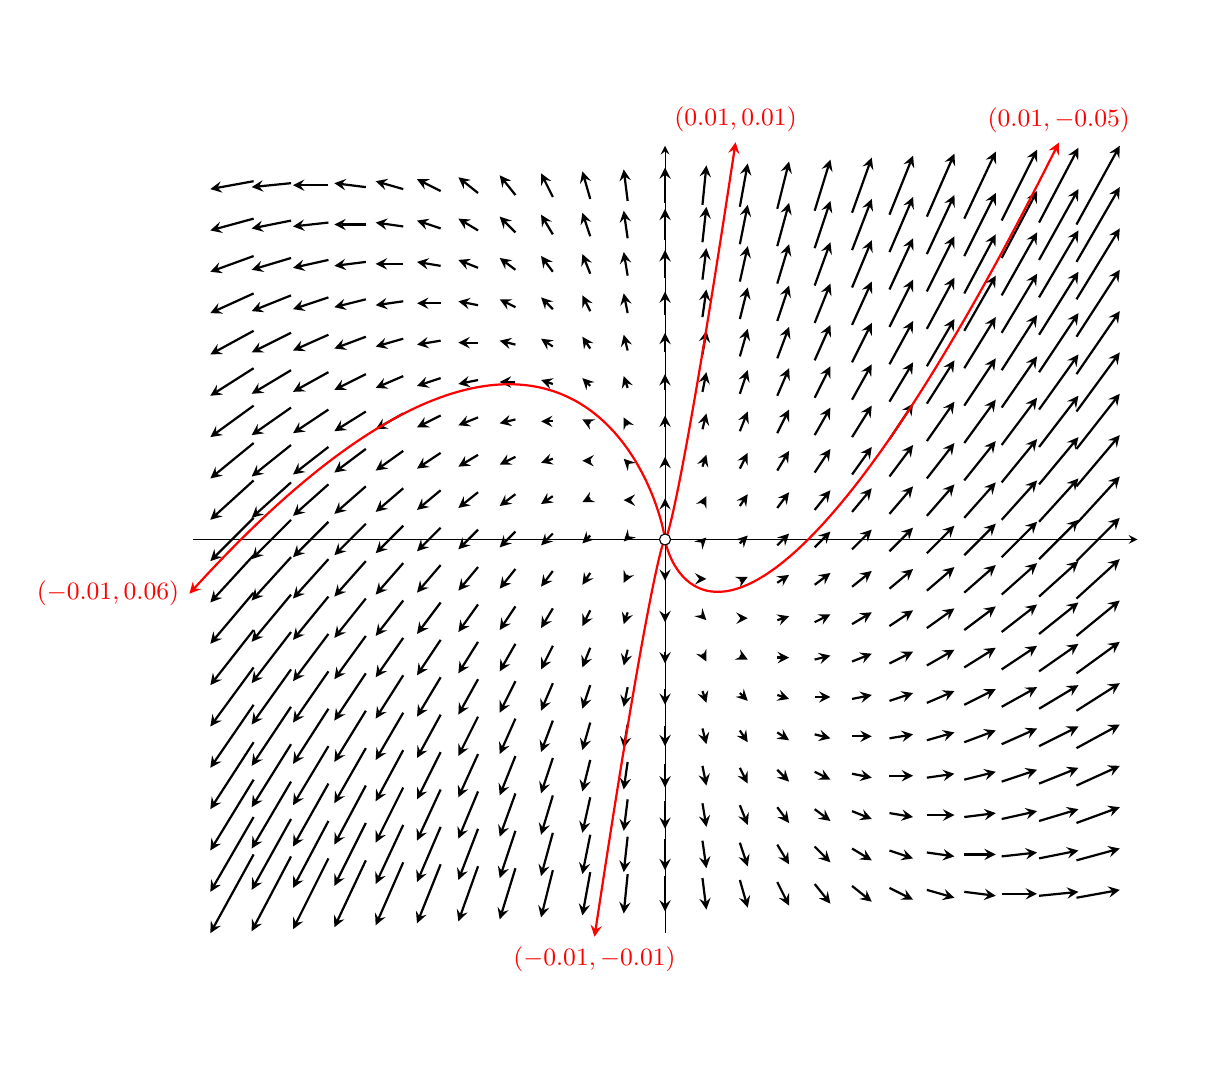
\begin{tikzpicture}[>=stealth]
	\def\xmin{-5.5}
	\def\ymin{-4.5}
	\def\xmax{5.5}
	\def\ymax{4.5}
	\draw[->] (-6,0)--(6,0);
	\draw[->] (0,-5)--(0,5);
	\def\s{0.1};
	\begin{scope}
		\clip (-0.2,-0.2)--(-0.2,0.2)--(0.2,0.2)--(0.2,-0.2)--(-0.2,-0.2)(-6.5,-6.5)--(6.5,-6.5)--(6.5,6.5)--(-6.5,6.5)--(-6.5,-6.5);
		\foreach \x in {-5.5,-5,...,5.5}{
			\foreach \y in {-4.5,-4,...,4.5}{
				\draw[->,thick] ({\x-(\s)*(\x)/2},{\y-(\s)*(\x+\y)/2})--({\x+(\s)*(\x)/2},{\y+(\s)*(\x+\y)/2});
			};
		};
	\end{scope}
	\foreach \x \y in {-0.01/-0.01,0.01/0.01,0.01/-0.05,-0.01/0.06}{
		\pgfmathsetmacro{\stepx}{0.01}
		\xdef\listdat{(\x,\y)}
		\pgfmathsetmacro{\myx}{\x}
		\pgfmathsetmacro{\myy}{\y}
		\foreach \k in {1,...,10000}{
			\pgfmathsetmacro{\myy}{\myy+(\myx+\myy)*\stepx}
			\pgfmathsetmacro{\myx}{\myx+\myx*\stepx}
			\xdef\myx{\myx}
			\xdef\myy{\myy}
			\xdef\listdat{\listdat (\myx,\myy)}
			\ifdim \myx pt < -6 pt
				\breakforeach
			\fi
			\ifdim \myx pt > 6 pt
				\breakforeach
			\fi
			\ifdim \myy pt < -5 pt
				\breakforeach
			\fi
			\ifdim \myy pt > 5 pt
				\breakforeach
			\fi
		}
		\ifdim \x pt > 0pt
			\draw[->,red,thick] plot[smooth] coordinates {\listdat}node[above]{\small{$(\x,\y)$}};
		\fi
		\ifdim \x pt < 0pt
			\ifdim \y pt > 0pt
				\draw[->,red,thick] plot[smooth] coordinates {\listdat}node[left]{\small{$(\x,\y)$}};
			\fi
			\ifdim \y pt < 0pt
				\draw[->,red,thick] plot[smooth] coordinates {\listdat}node[below]{\small{$(\x,\y)$}};
			\fi
		\fi
	}
	\draw[fill=white] (0,0)circle(2pt);
\end{tikzpicture}
\end{document}
